\subsection{Actividad 11}
Simular en \textsc{SIMULINK} los sistemas de control PID
discreto de los apartados 9. y 10. usando los parámetros
correspondientes, añadiendo asimismo una limitación de salida del
controlador discreto a $(-15,+15)$ añadiendo en su caso el sistema
corrector anti-windup y ver la respuesta ante ángulo de consigna
escalón unitaria, graficando asimismo la señal de control.

\begin{tcolorbox}[sharp corners, colframe=bluebox, title= Simulink PD]
  \mkanscode{
\begin{figure}[H]
  \centering
  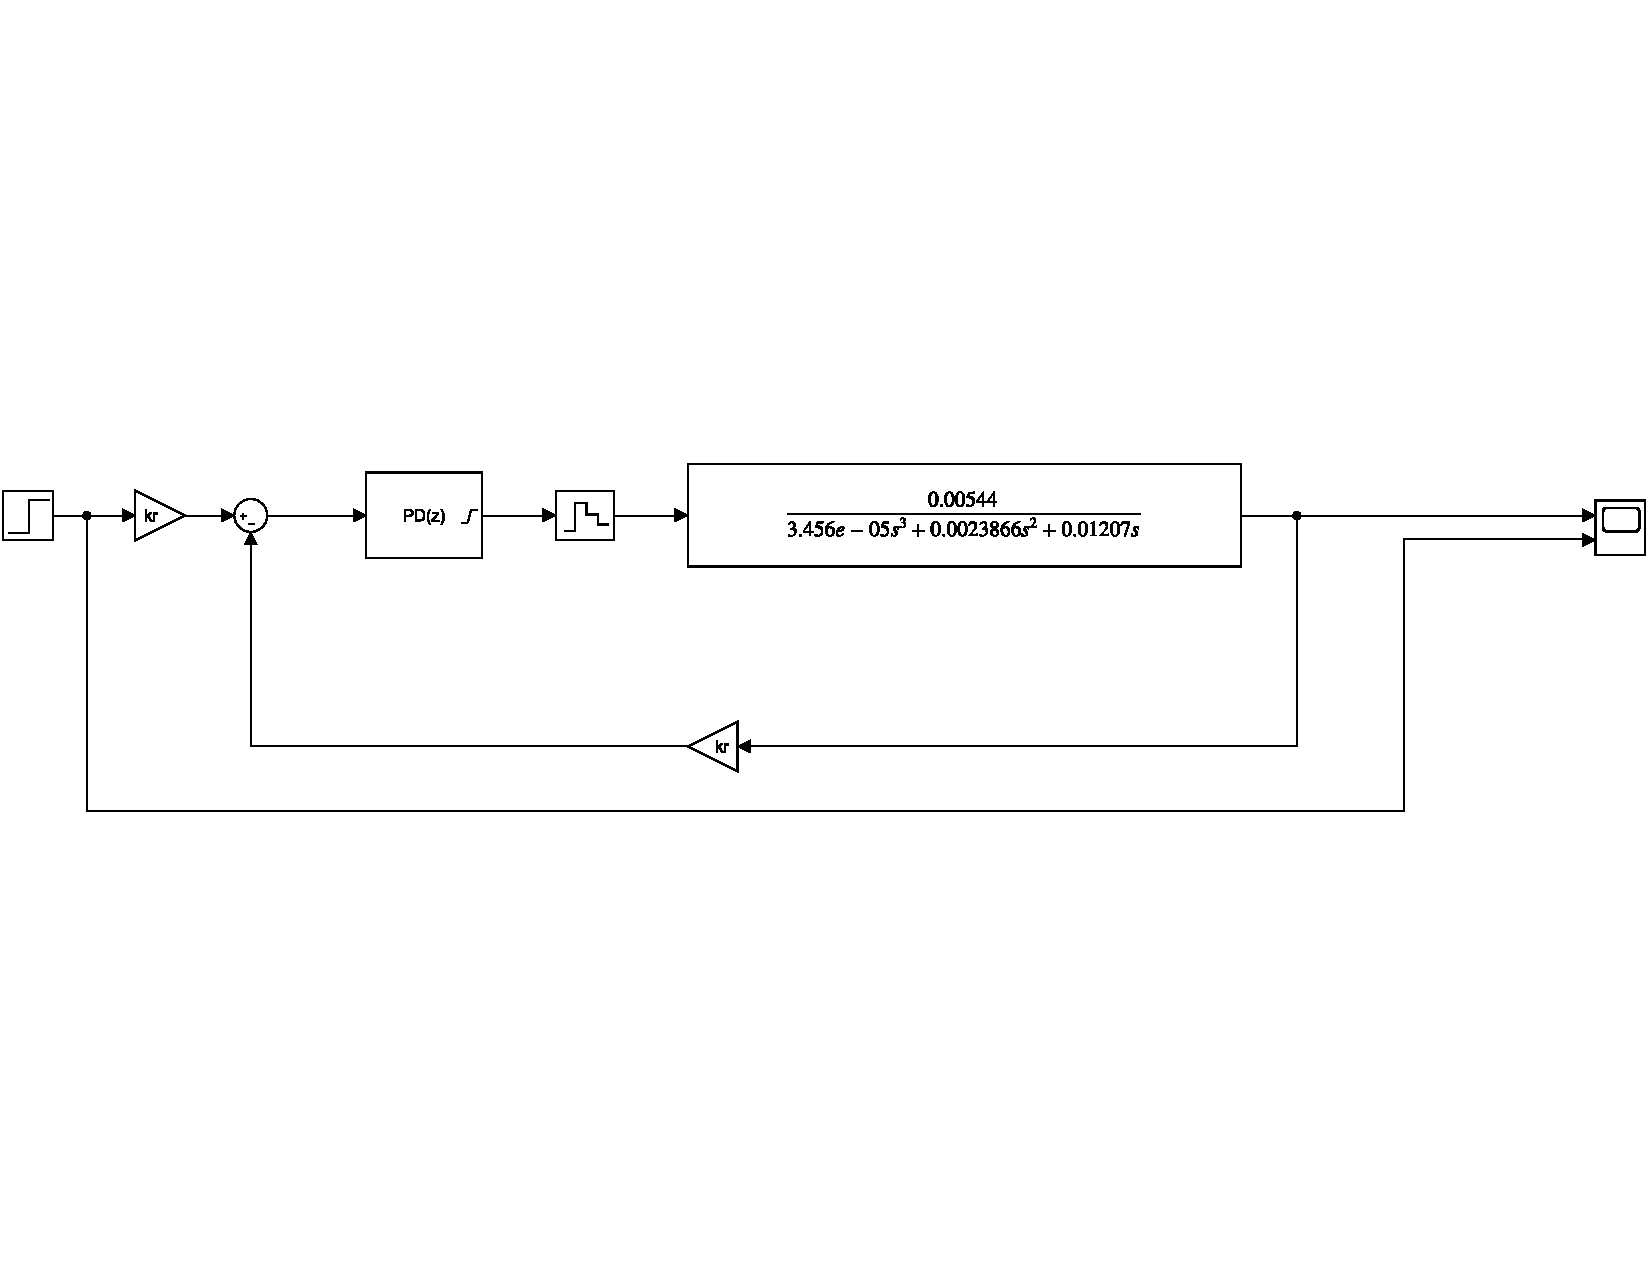
\includegraphics[clip, trim=0cm 6cm 0cm 6cm,scale=0.48]{images/figura 11.pdf}
  % izquierda,abajo,derecha,arriba
  \caption{Simulink - Diagrama de bloques.}
    \label{fig:figura 11}
\end{figure}
}

\begin{tcolorbox}[sharp corners, colback = white]
    \color{gray}
\begin{verbatim}
Use filtered derivative
    Filter coefficient (N): 45
Upper limit: 15
Lower limit: -15 
\end{verbatim}
  \end{tcolorbox}%
\vspace*{0.5em}
  \mkanscode{
\begin{figure}[H]
  \centering
  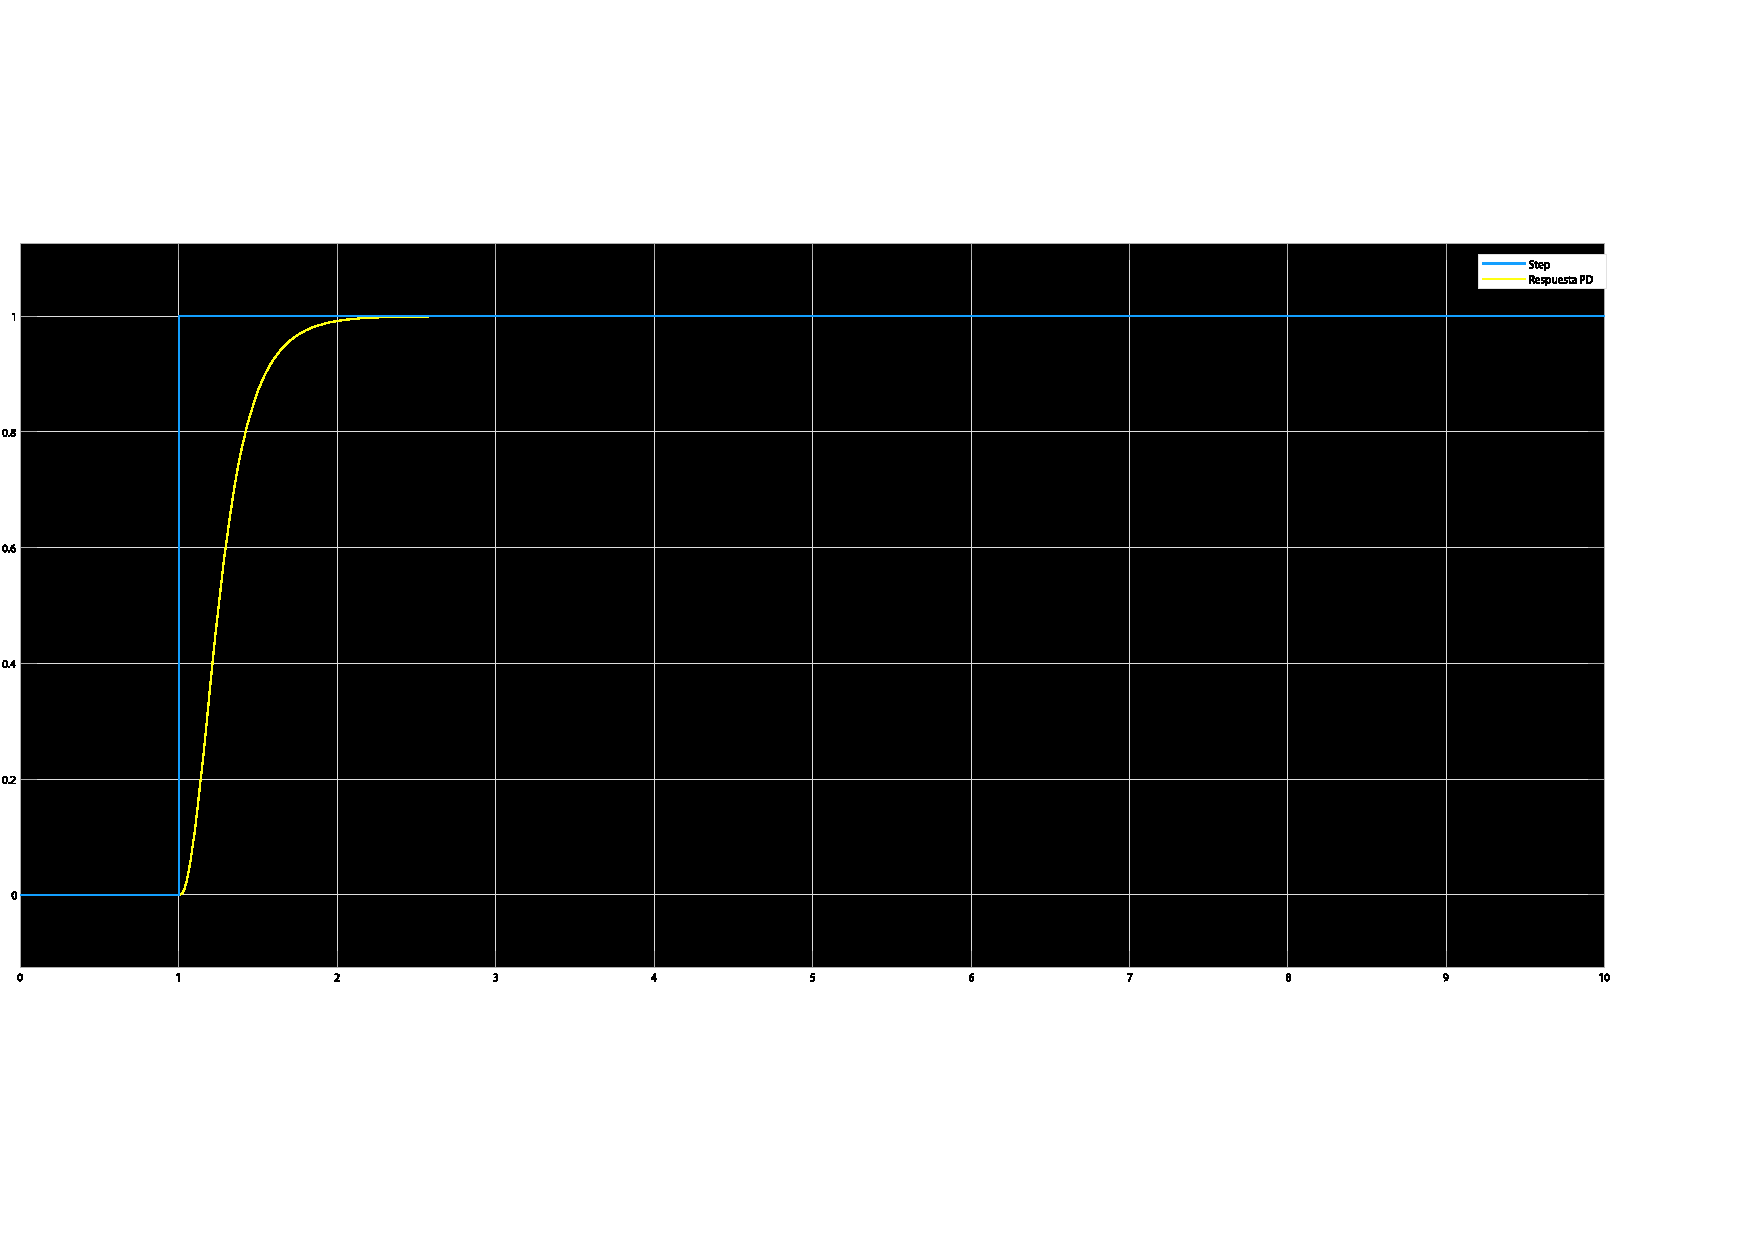
\includegraphics[clip, trim=0cm 4cm 0.90cm 4cm,scale=0.48]{images/figura 12.pdf}
  % izquierda,abajo,derecha,arriba
  \caption{Simulink - Respuesta a un escalón.}
    \label{fig:figura 12}
\end{figure}
  }
\end{tcolorbox}%

\begin{tcolorbox}[sharp corners, colframe=bluebox, title= Simulink PID,breakable=unlimited]
  \mkanscode{
\begin{figure}[H]
  \centering
  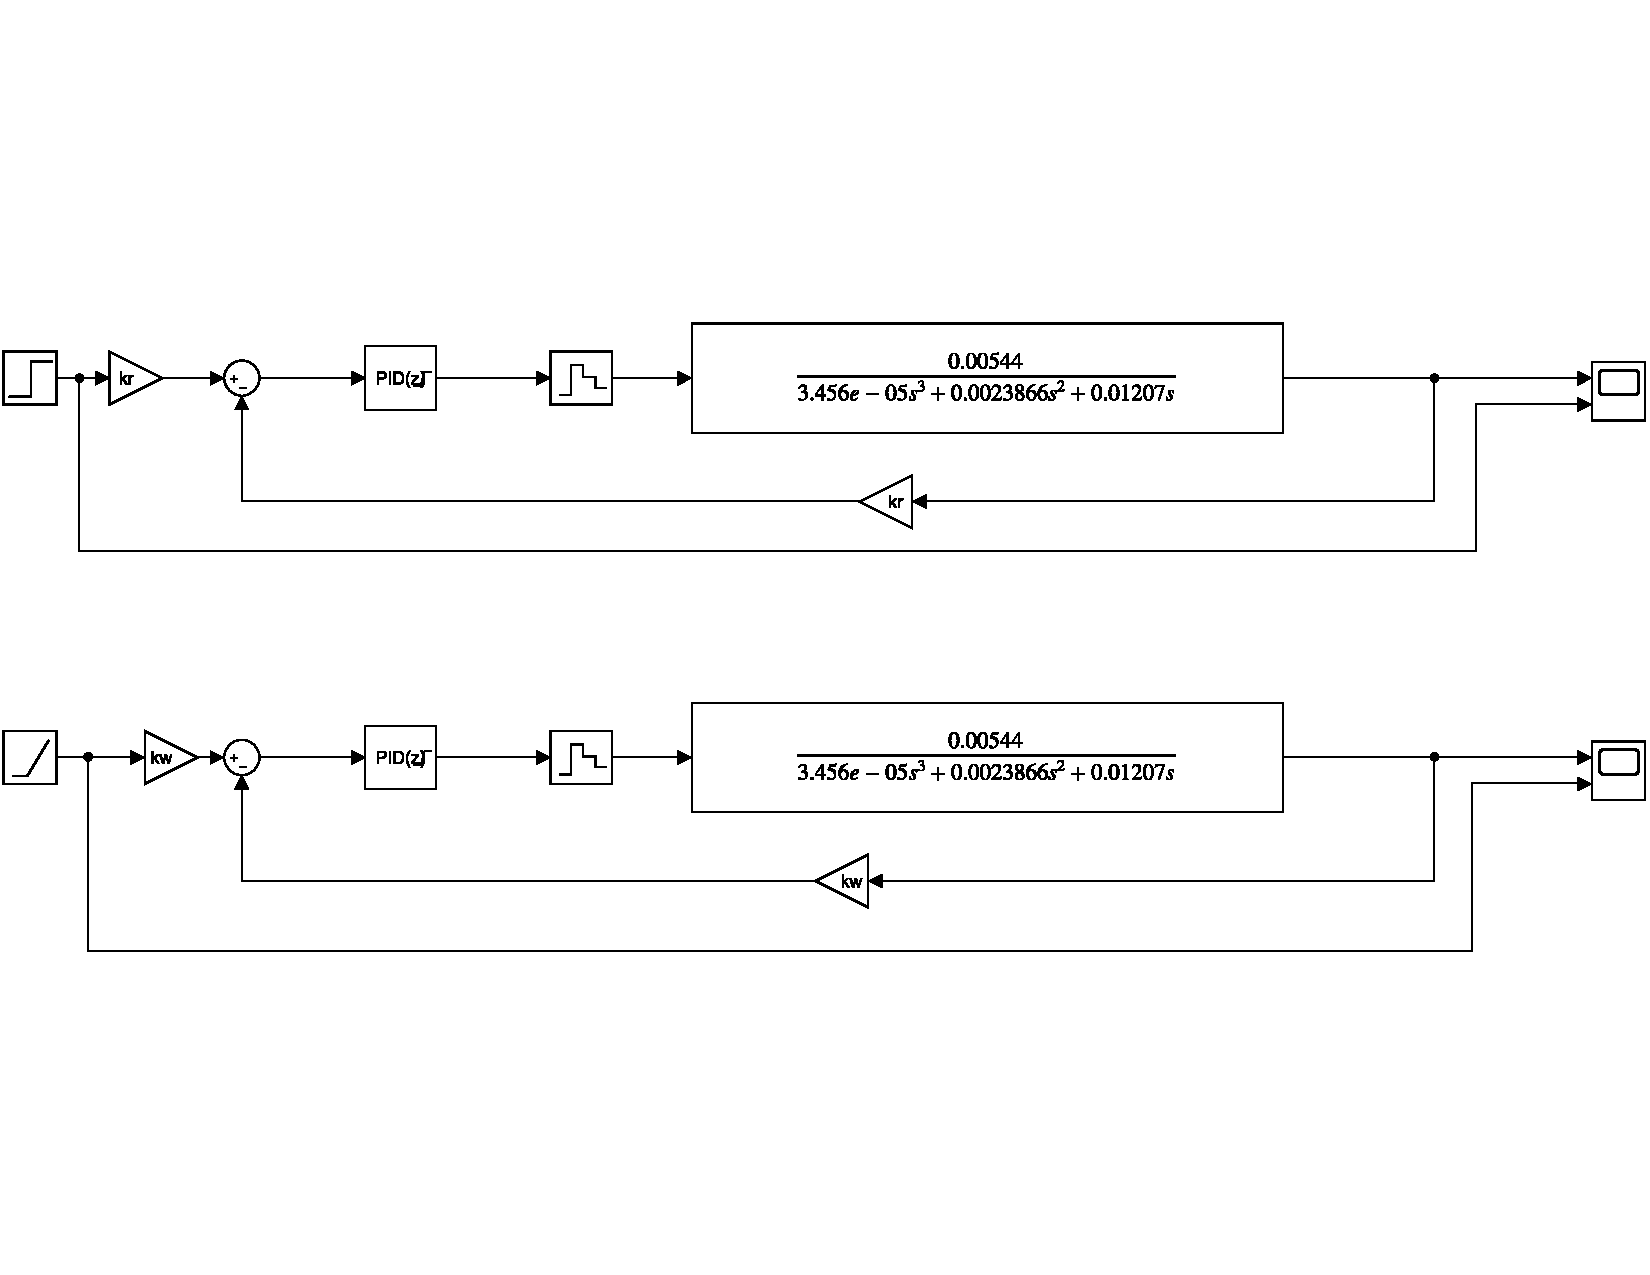
\includegraphics[clip, trim=0cm 5.35cm 0cm 5.34cm,scale=0.48]{images/figura 13.pdf}
  % izquierda,abajo,derecha,arriba
  \caption{Simulink - Diagrama de bloques.}
    \label{fig:figura 13}
\end{figure}
}

\begin{tcolorbox}[sharp corners, colback = white]
    \color{gray}
\begin{verbatim}
Use filtered derivative
    Filter coefficient (N): 45
Upper limit: 15
Lower limit: -15 
Anti-windup Method: Campling
\end{verbatim}
  \end{tcolorbox}%
\vspace*{0.5em}
  \mkanscode{
\begin{figure}[H]
  \centering
  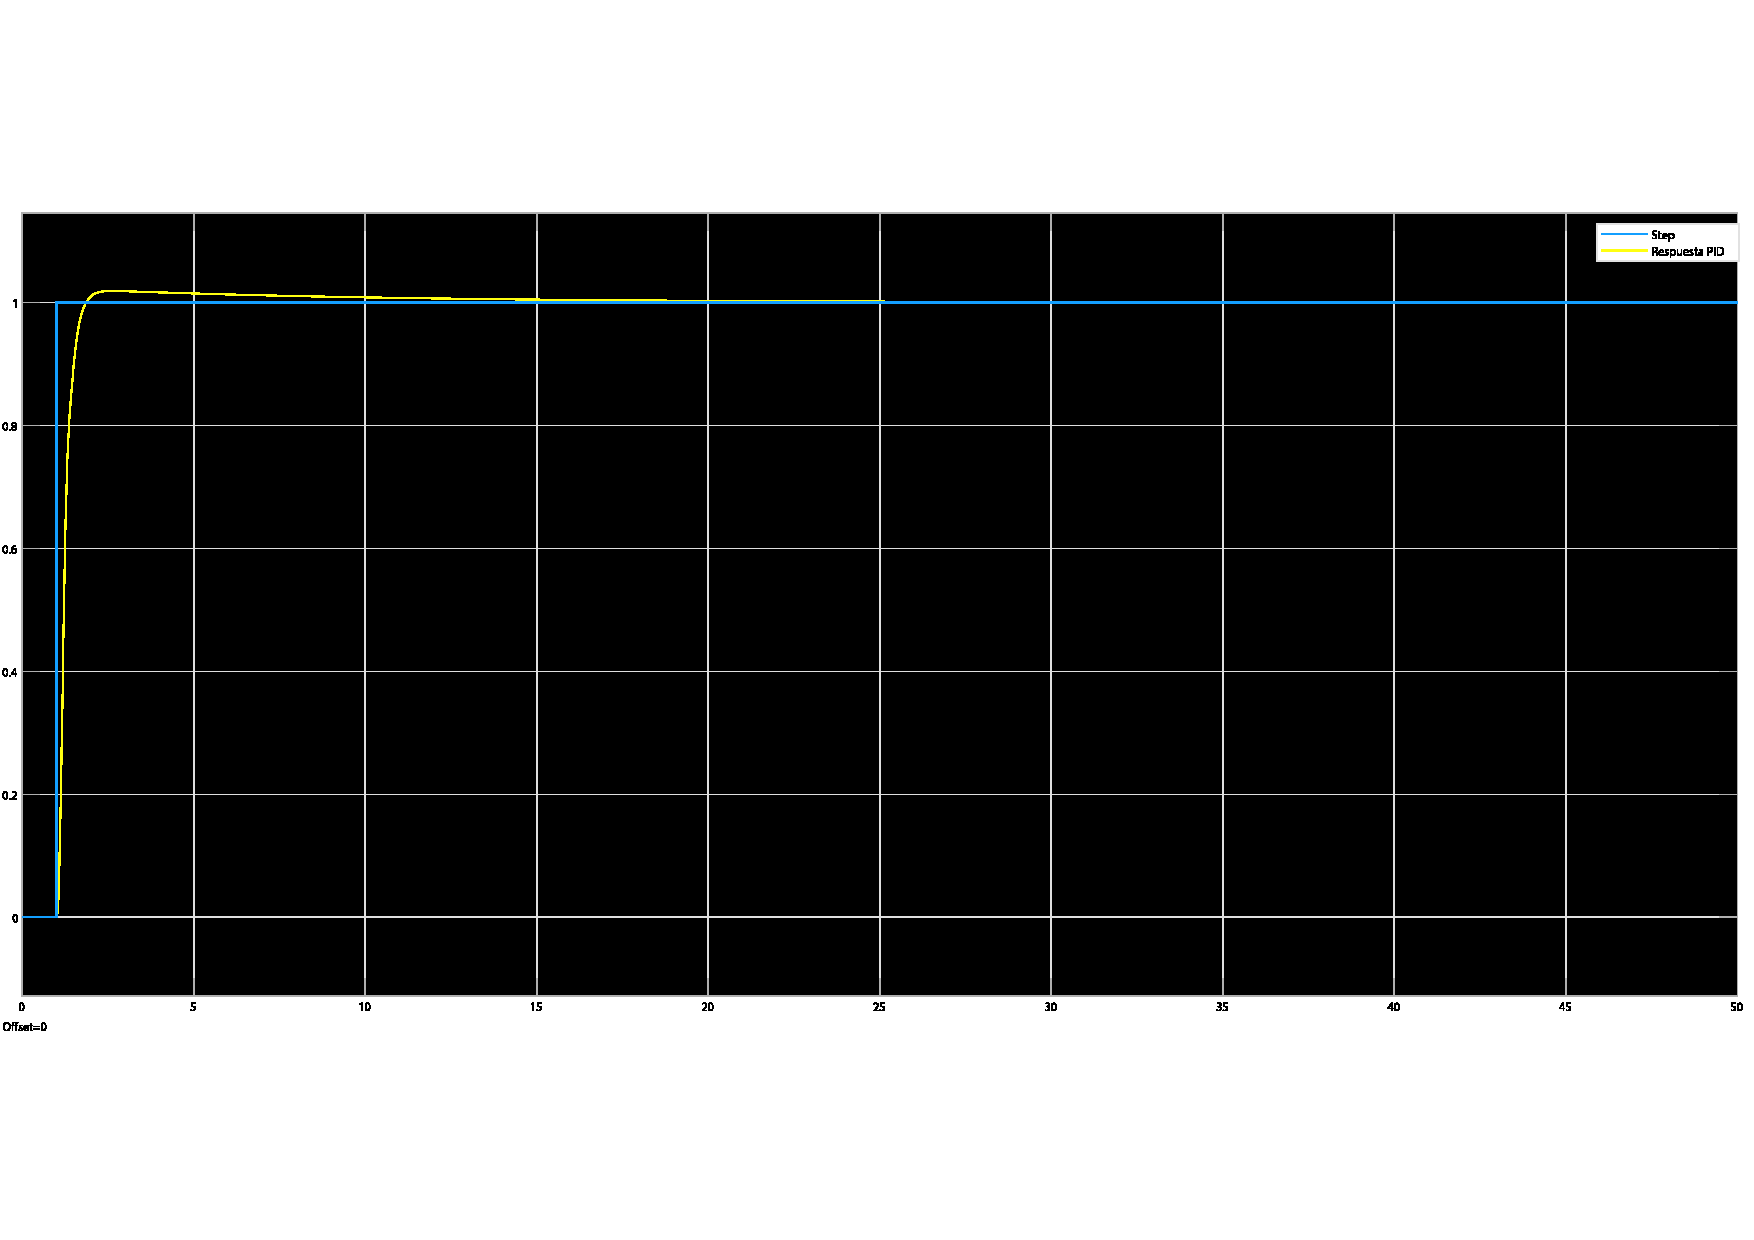
\includegraphics[clip, trim=0cm 3.7cm 0cm 3.7cm,scale=0.48]{images/figura 14.pdf}
  % izquierda,abajo,derecha,arriba
  \caption{Simulink - Respuesta a un escalón.}
    \label{fig:figura 14}
\end{figure}
}
\vspace*{0.5em}
  \mkanscode{
\begin{figure}[H]
  \centering
  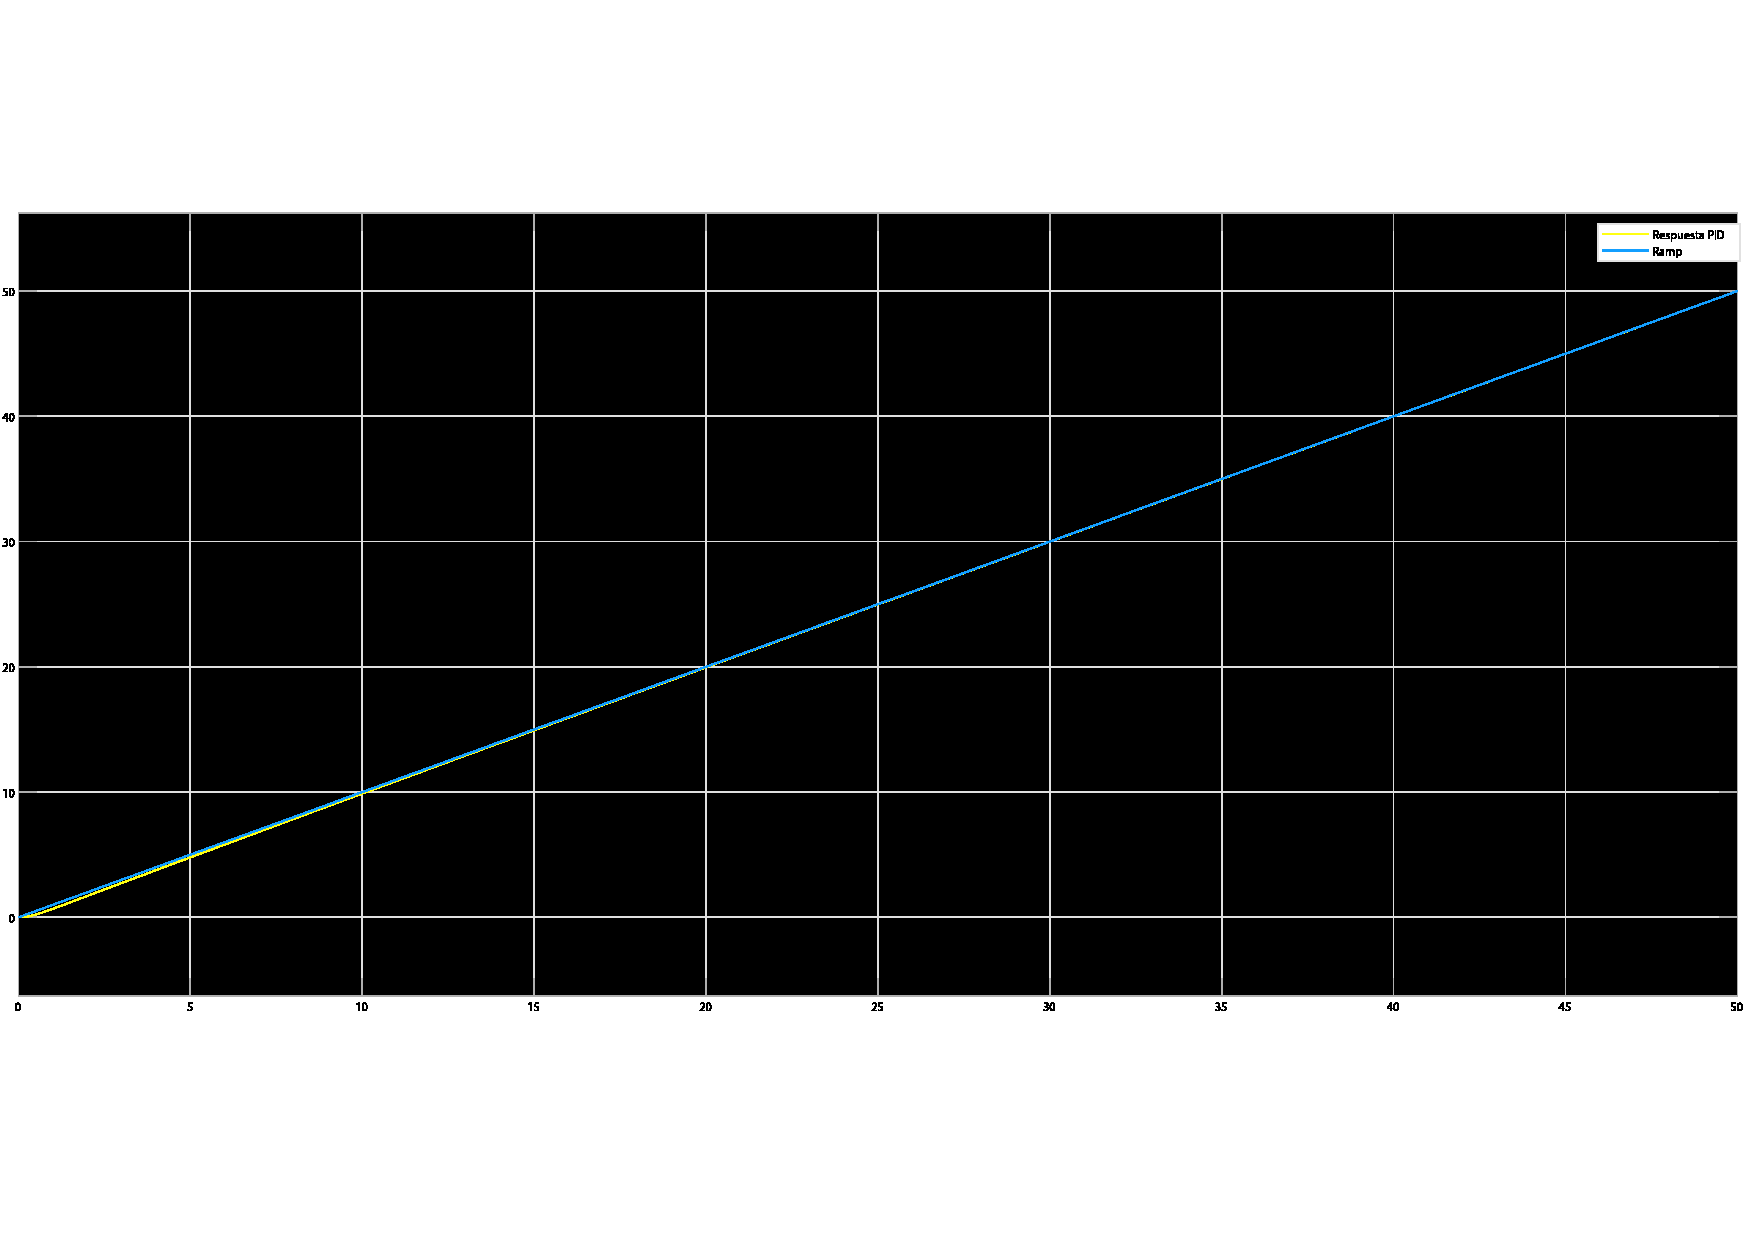
\includegraphics[clip, trim=0cm 3.7cm 0cm 3.7cm,scale=0.48]{images/figura 15.pdf}
  % izquierda,abajo,derecha,arriba
  \caption{Simulink - Respuesta a una rampa.}
    \label{fig:figura 15}
\end{figure}
  }
  \end{tcolorbox}%